%% Paper I of the split of docs/paper1 (docs/split_paper_tasks.md): dynamics and transfer.
%% Target: Chaos (S0.2); drafted in the AGU class like paper1, REVTeX at S3.14.
\PassOptionsToPackage{natbibapa}{apacite}% keep \citet / \citep with apacite
\documentclass[draft]{PJ2019}

\usepackage{amsmath,amssymb}
\usepackage{amsthm}
\usepackage{mathtools}
\usepackage{bm}
\usepackage{booktabs}
\usepackage{xcolor}
\usepackage{xspace}
\usepackage[group-separator={,}]{siunitx}
\usepackage[hidelinks]{hyperref}

% Shared notation; copied from docs/paper1/macros.tex at the split (S1.5).
\newcommand{\DKY}{D_{\mathrm{KY}}}
\newcommand{\dlat}{d_{\mathrm{lat}}}
\newcommand{\Nens}{N_{\mathrm{ens}}}
\newcommand{\R}{\mathbb{R}}
\newcommand{\Z}{\mathbb{Z}}
\newcommand{\E}{\mathcal{E}}          % encoder
\newcommand{\Dec}{\mathcal{D}}        % decoder
\newcommand{\Fp}{\mathcal{F}}         % latent propagator
\newcommand{\Hobs}{\mathcal{H}}       % physical observation operator
\newcommand{\Lat}{\Lambda}            % site lattice
\newcommand{\Shift}{\mathsf{S}}       % lattice shift
\newcommand{\Tr}{\mathsf{T}}          % physical translation
\newcommand{\Exp}{\mathbb{E}}
\newcommand{\Var}{\operatorname{Var}}
\newcommand{\Cov}{\operatorname{Cov}}
\newcommand{\tr}{\operatorname{tr}}
\newcommand{\dist}{\operatorname{dist}}
\newcommand{\Renc}{R_{\mathrm{enc}}}
\newcommand{\Rdec}{R_{\mathrm{dec}}}
\newcommand{\Rprop}{R_{\mathrm{prop}}}
\newcommand{\kmax}{k_{\max}}
\newcommand{\kmid}{k_{\mathrm{mid}}}
\newcommand{\wvar}{w_{\mathrm{var}}}
\newcommand{\wld}{w_{\mathrm{ld}}}
\newcommand{\ie}{i.e.\@\xspace}
\newcommand{\eg}{e.g.\@\xspace}

\newtheorem{proposition}{Proposition}
\newtheorem{lemma}{Lemma}
\newtheorem{corollary}{Corollary}
\theoremstyle{remark}
\newtheorem{remark}{Remark}

% Run-in paragraph heading (revtex letters \paragraph headings; we do not want that).
\newcommand{\para}[1]{\par\medskip\noindent\textbf{#1}\enspace}

% Wide table: full line width with the columns spread out (like revtex's ruledtabular) when it fits,
% shrunk to the line width only when its natural width is larger -- never enlarged, so a narrow table
% keeps the float font size (fixed 2026-10-11: \resizebox alone scaled small tables up).
% #1: column spec, #2: body (header + rows). The body is typeset twice (measured, then set).
\makeatletter
\newsavebox\wt@box
\newcommand{\widetabular}[2]{%
  \sbox\wt@box{\begin{tabular}{#1}\hline\hline\noalign{\vskip 2pt}#2\noalign{\vskip 2pt}\hline\hline\end{tabular}}%
  \ifdim\wd\wt@box>\linewidth
    \resizebox{\linewidth}{!}{\usebox\wt@box}%
  \else
    \begin{tabular*}{\linewidth}{@{\extracolsep{\fill}}#1}\hline\hline\noalign{\vskip 2pt}#2\noalign{\vskip 2pt}\hline\hline\end{tabular*}%
  \fi}
\makeatother
% Table bodies are read with TeX's primitive \input (expandable), so a rule may follow them.
\makeatletter\newcommand{\tabinput}[1]{\@@input #1.tex }\makeatother

% REVTeX's ruledtabular (used by every table) for non-REVTeX classes: centred table with
% double rules above and below; the table body supplies its own \hline after the header.
\makeatletter
\@ifundefined{ruledtabular}{%
\newenvironment{ruledtabular}{\par\centering
  \let\rt@tabular\tabular \let\rt@endtabular\endtabular
  \renewenvironment{tabular}[1]{\rt@tabular{##1}\hline\hline\noalign{\vskip2pt}}%
    {\noalign{\vskip2pt}\hline\hline\rt@endtabular}}{\par}}{}
\makeatother

% Placeholder for numbers that pending runs will fill (Block K; see docs/paper1/partII_narrative.md,
% table P1-P12). Renders in red so none survives into a submitted draft unnoticed.
\providecommand{\textcolor}[2]{#2}
\newcommand{\placeholder}[1]{\textcolor{red}{\textbf{[#1]}}}


% Float placement for a single-column draft: let figures and tables sit near their first
% mention (the REVTeX top-only placement pushed most of them to the end of the paper).
\renewcommand{\topfraction}{0.9}
\renewcommand{\bottomfraction}{0.8}
\renewcommand{\textfraction}{0.07}
\renewcommand{\floatpagefraction}{0.75}
\setcounter{topnumber}{3}
\setcounter{bottomnumber}{2}
\setcounter{totalnumber}{5}

\journalname{Draft}

\begin{document}

\title{Local latent fields for extensive spatiotemporal chaos: zero-shot domain transfer
validated by Lyapunov spectra}

\authors{Dalton Jones\affil{1}, Peter Jan van Leeuwen\affil{1}}

\affiliation{1}{Department of Atmospheric Science, Colorado State University, Fort Collins, USA}

\correspondingauthor{Dalton Jones}{daltjone@colostate.edu}

% Key points: AGU limit of three, at most 140 characters each, no special characters.
\begin{keypoints}
\item A learned local latent field trained at one domain size reproduces the true Lyapunov dimension on domains up to four times larger.
\item Training on windows of one large simulation, with boundaries driven by the simulation, is what lets the learned local rule transfer.
\item Training rollouts that are too short or too long distort the learned chaos; a rule that uses no ground truth picks a good model.
\end{keypoints}

% Every number below is in a table: Table~\ref{tab:transfer1d} (1D), Table~\ref{tab:transfer2d} (2D),
% Table~\ref{tab:architecture} (parameters); the box-trained range in Fig.~\ref{fig:box_vs_window}
% and App. D; the selection rule in Sec.~\ref{sec:canonical_results}.
\begin{abstract}
Learned surrogates of spatiotemporally chaotic systems usually compress the state into one latent
vector whose size is fixed at training time, although in extensive chaos the number of active
degrees of freedom grows with the domain. We make the latent a field: a few channels at each site of
a lattice that tiles the domain, built only from weight-shared operators of finite reach, so that one
model, of about $135{,}000$ parameters in 2D, runs on any larger domain by adding sites. Judged by its
own Lyapunov spectrum, a one-dimensional Kuramoto--Sivashinsky model trained at $L=100$ reproduces
the Kaplan--Yorke dimension to within $0.2$--$1.2\%$ up to $L=400$. In two-dimensional
Kuramoto--Sivashinsky and Kolmogorov flows, models trained on a small periodic box miss the
dimension of larger domains by up to $38\%$, while models trained on windows of one large
simulation, with driven boundaries, are within $0.6$--$2\%$ in Kuramoto--Sivashinsky and $1$--$9\%$
in Kolmogorov flow at the two stronger drags. We prove that this window training is exactly the
training of a limited-area model. Two further choices in training can make a learned local rule fail: rollouts
that are too short admit spurious free-running regimes, and squared-error rollouts that are too
long damp the growth rates, a bias that follows from the structure of the loss. Free-rollout
statistics compared with the training data detect the first problem without any ground truth, and
a selection rule built on them chose, among six variants, the one with the lowest mean error.
\end{abstract}

\section*{Plain Language Summary}
Many chaotic systems, from flame fronts to atmospheric flows, are spatially extended: the
larger the domain, the more independent chaotic degrees of freedom it holds. Machine-learned
surrogates usually describe the whole state by one fixed-length list of numbers, which cannot
grow with the domain. We instead learn a field of a few numbers at each point of a lattice,
updated by the same local rule everywhere, so that a model trained on a small domain runs on a
larger one simply by adding lattice points. We check this transfer with the strictest test
available, the model's own Lyapunov spectrum against that of the true equations, in three
systems. What makes the learned rule transfer is the data it is trained on: pieces of one large
simulation rather than a small closed box. We also show which training choices make the learned
chaos too weak or send it into the wrong state, and how to detect the second without knowing the
answer.

%======================================================================
\section{Introduction}
\label{sec:introduction}
%======================================================================

Learned surrogates of chaotic partial differential equations usually
compress the whole state into one latent vector and learn how that
vector evolves \citep{linotgraham2022,racca2023,ozalpmagri2025}. For
many systems this is the right design. For spatiotemporally chaotic
systems on large domains it is not, for a reason that is structural
rather than technical. Such systems are extensively chaotic: the number
of active degrees of freedom, measured by the Kaplan--Yorke dimension
$\DKY$, grows in proportion to the domain
\citep{ruelle1982,manneville1985,egolfgreenside1994}. A latent vector
fixed at training time has no size to grow into. A model trained on one
domain cannot even be evaluated on another, and every new domain size
requires new data and new training.

We study the alternative: a latent \emph{field}, with a few channels at
each site of a lattice that tiles the physical domain, built only from
operators that are shared by all sites and read a bounded neighbourhood
(Fig.~\ref{fig:concept}).
The parameters of such a model do not depend on the number of sites, so
a model trained at one size is applied to a larger domain by adding
sites, with no retraining. Its latent also has a physical geometry, which
a companion paper uses to build a localized ensemble filter in latent space
\citep{jones2026da}. A local, weight-shared model is
also extensive by construction, like the coupled lattice maps whose
Lyapunov spectra have a thermodynamic limit \citep{livi1986,isola1990}
and can be predicted from small subsystems \citep{carretero1999}. The
question is whether a \emph{learned} local rule reproduces the right
density of chaos, and whether it keeps doing so on domains it was never
trained on.

Two things turn out to matter, and they organize the paper. First, the
data the local rule is learned from. A rule of finite reach can be
learned from a small periodic box, or from windows of one large
simulation, by the same procedure: in both, the sites that border the
scored region are overwritten with data at every step, so the training
loss is that of a limited-area model. Trained on a small box, the rule
transfers in the Kuramoto--Sivashinsky (KS) equation, in
one and in two dimensions. In Kolmogorov flow it transfers only while
the larger domain's large-scale motion stays like the box's; beyond
that, the transferred model drifts into a state with far too much
large-scale energy, and windows of a large simulation are needed.
Second, the propagator must stay chaotic when it runs freely: rollouts
that are too short admit spurious regimes, and longer squared-error
rollouts lower the dimension.

We hold the models to a demanding standard: their own Lyapunov spectra,
computed from the learned maps, compared with spectra of the true PDE at
every domain size, with the uncertainty of the reference measured rather
than assumed. We do this for the one-dimensional KS equation, its two-dimensional
isotropic form, and two-dimensional Kolmogorov flow with linear drag at
three drag coefficients.

\begin{figure*}[htbp]
\centering
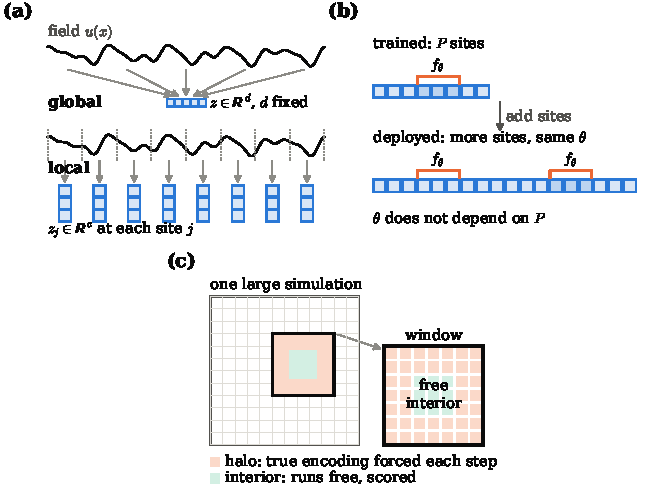
\includegraphics{figures/concept_transfer.pdf}
\caption{The idea in three panels. (a) A global latent compresses the
whole field into one vector of fixed dimension $d$; a local latent field
assigns $c$ channels to the site of each patch. (b) Because every
operator is shared across sites and reads a bounded neighbourhood, the
trained parameters $\theta$ do not depend on the number of sites, and the
model is deployed on a larger domain by adding sites. (c) Training with
a forced halo: at every step of a training rollout the halo of the
window is overwritten by the true encoding, the interior runs free, and
only the interior is scored, so the loss is exactly that of a
limited-area model (Proposition~\ref{prop:halo}). The window can be cut
from one large simulation, as drawn, or be a small periodic box itself
(Sec.~\ref{sec:crop_training}).}
\label{fig:concept}
\end{figure*}

\para{Contributions.}
\begin{itemize}
\item \emph{A local latent field for extensive chaos}
  (Sec.~\ref{sec:method}): weight-shared encoder, decoder and propagator
  of finite reach, equivariant under shifts by whole patches, with a
  parameter count independent of the domain size: $76{,}000$--$135{,}000$
  parameters describe the local law once, and the same parameters run
  domains of any size.
\item \emph{One training procedure, two routes}
  (Sec.~\ref{sec:crop_training}): a forced halo, overwritten with data at
  every step of a training rollout, makes the training loss that of a
  limited-area model, whether the window is a small periodic box or a
  piece of one large simulation.
\item \emph{Zero-shot transfer validated by Lyapunov spectra}
  (Secs.~\ref{sec:results1d} and~\ref{sec:results2d}). Trained at $L=100$,
  a 1D KS model reproduces the true $\DKY$ to within $0.2$--$1.2\%$ from
  $L=50$ to $L=400$, and its whole positive spectrum collapses onto the
  truth's. Trained on a $44^2$ periodic box, three 2D KS models are within
  $3.5\%$ of the truth at $44^2$ and $66^2$, a size never seen in training.
  In 2D the leading exponent is $12$--$30\%$ too high, which we report
  alongside $\DKY$.
\item \emph{Where a small box stops being enough}
  (Sec.~\ref{sec:kolm_box}): in Kolmogorov flow the small-box model fails
  where the truth's large-scale energy grows beyond what the box contains,
  at three times the box width at the strongest drag and at twice it at a
  weaker one. Trained on windows of a simulation sixteen boxes wide, the
  same architecture is within $10\%$ at the two stronger drags.
\item \emph{What fails, and why} (Sec.~\ref{sec:failure}): softmax
  attention, short rollouts and the damping of $\DKY$ by long
  squared-error rollouts, which we connect, as a hypothesis, to the law of
  total variance.
\end{itemize}

What is not new should be said as clearly. Localized reduced models of KS
were built from wavelets a quarter century ago \citep{wittenberg2001},
learned models of KS have reproduced Lyapunov spectra at a single size
\citep{pathak2017,vlachas2020,ozalpmagri2025}, and convolutional
surrogates have been run on larger domains than they were trained on
\citep{barsinai2019,kochkov2021}. Section~\ref{sec:background} places our
results among these. The contrast with minimal flow units, which are
non-extensive by construction and where a global latent vector works
well \citep{constanteamores2025}, is the one-sentence summary of when a
field-valued latent is needed.

Section~\ref{sec:method} defines the model, its structural properties and
the training rule; Section~\ref{sec:systems} describes the three systems
and how precisely their Lyapunov spectra are known.
Sections~\ref{sec:results1d} and~\ref{sec:results2d} report transfer in
one and two dimensions, Section~\ref{sec:failure} the failure modes, and
Section~\ref{sec:discussion} what transfer requires and the limitations
of this study.

%======================================================================
\section{Background}
%======================================================================
% TODO(S3.3): paper1 §2.1, §2.2, §2.4 + Table 1 without the local-DA column.
\placeholder{S3.3: Background}

%======================================================================
\section{Method}
%======================================================================
% TODO(S3.4): paper1 §3.1--3.7 (no §3.8).
\placeholder{S3.4: Method}

%======================================================================
\section{Systems and ground truth}
%======================================================================
% TODO(S3.5): paper1 §4.
\placeholder{S3.5: Systems and ground truth}

%======================================================================
\section{Transfer in one dimension}
%======================================================================
% TODO(S3.5): paper1 §5.
\placeholder{S3.5: Transfer in one dimension}

%======================================================================
\section{Transfer in two dimensions}
%======================================================================
% TODO(S3.5): paper1 §6 (per-patch paragraph: one pointer to Paper II).
\placeholder{S3.5: Transfer in two dimensions}

%======================================================================
\section{Failure modes}
%======================================================================
% TODO(S3.5): paper1 §8.
\placeholder{S3.5: Failure modes}

%======================================================================
\section{Discussion and limitations}
\label{sec:discussion}
%======================================================================

\para{What transfer requires.} Four conditions emerged, and each was
necessary in at least one system. First, the physics must be extensive
at the scales involved, which can be checked from ground truth at two
sizes before any model is trained: the 2D KS density is constant within
the spread of the truth runs ($82.0$ and $84.0$ per base box at $44^2$ and
$66^2$), while in Kolmogorov flow the truth's density per box rises with
the channel width at every drag (Table~\ref{tab:truth}). A local model
is extensive by construction (Remark~\ref{rem:extensive_model}), so
wherever the truth is not, a transfer error is expected and is not a
failure of training. Second, the training data must contain the local
statistics of a large domain: trained on a small periodic box the same
architecture misses $\DKY$ by $15$--$38\%$ in three of four larger
configurations, and trained on windows of one large simulation it
transfers (Sec.~\ref{sec:box_vs_window}); the window training is a
limited-area problem, and Proposition~\ref{prop:halo} shows that the
forced halo trains exactly that problem. Third, the learned map must
remain chaotic, and chaotic at the right rate, when it runs freely
(Secs.~\ref{sec:fail_regimes} and \ref{sec:fail_mse}); free-rollout
statistics detect spurious regimes without any truth, and the truth-free
selection rule of Sec.~\ref{sec:canonical_results} chose a model within
$0.9$--$5.9\%$ of the truth at every width. Fourth, the model's reach must
cover the interaction range of the dynamics.

\para{The interaction range is the design length.} The light cone is far
too short to constrain the reach of a model at these time steps; the
length that matters is the distance beyond which neighbouring values stop
improving a one-step prediction, three to four sites for the 1D latent
dynamics against a trained reach of six (Sec.~\ref{sec:receptive}). In
Kolmogorov flow most of the unstable directions lie in the band around
the forcing wavenumber, $31.5$ of $36$ at $|\bm k|\in[2,8)$ for $\alpha=0.05$ at
$3\times$, whose wavelengths span one to four sites, and a model of finite
reach reproduces this scale content (Appendix~\ref{app:chaos_scale}). Models whose encoder
reaches two sites and whose propagator reaches one fail even when trained
on windows of the very domain they are evaluated on, with errors of
$66$--$100\%$ in $\DKY$ (Appendix~\ref{app:tables}). The rule we take from
this is to measure the interaction range on data, for example by fitting
a shared stencil of increasing width, and to give the encoder and
propagator a reach that covers it with a margin. The reach then sets the
smallest domain the model can be used on, which is what fails at $L=25$.

\para{The parameters describe the law, not the state.} Because every
operator is shared by all sites, the trained parameters encode one local
rule, and their number is fixed by that rule rather than by the domain.
A 2D model of about $135{,}000$ parameters reproduces a Kaplan--Yorke
dimension of $188$ at $66^2$ to within $0.6\%$ (Table~\ref{tab:transfer2d}), and
a 12-channel version runs a $440^2$ domain, whose attractor dimension we
estimate at roughly $8{,}000$ from the measured density of $0.043$ per unit area
\citep{jones2026da}. The same weight sharing makes training cheap in
data: every window, and every site within it, is a training example of
the same rule. Weight sharing and size independence are not new by
themselves \citep{barsinai2019,kochkov2021}; what the dimension comparison
adds is evidence that the shared rule is the right one, in the sense that
its extension to a larger domain carries the right density of chaos. A
system made of many copies of one local process is described most
economically by learning that process once.

\para{Transfer error as a probe of the physics.} Because a local model
is extensive by construction, the difference between its dimension
density and the truth's on a larger domain measures how far the truth is
from extensive at that size, once the model is accurate at the native
size. The weakest drag, where the native-size models scatter most and the
transferred models fall below a rising truth, is where the inverse
cascade is least arrested, and we expect non-local effects to be largest
there. Using
transfer error to locate the scales at which a system stops being
extensive is a question in its own right, which we leave to future work.

\para{Limitations.} We state them plainly.
\begin{itemize}
\item \emph{Ground truth.} Five Kolmogorov configurations rest on one 40-unit
  run, uncertain by 10--15\%, the 2D KS truths by a few percent
  (Sec.~\ref{sec:truth_uncertainty}), and there is no truth at $88^2$.
\item \emph{Kolmogorov geometry.} The channel is widened in $x$ only,
  because the forcing fixes the height; transfer in $y$ is untested.
\item \emph{Models.} Most 2D models have one training seed (the 1D model
  has three, the $\alpha=0.05$ canonical model two); the 1D and 2D
  canonical architectures differ (full reach in 1D, per-patch in 2D); the
  weakest drag remains $8$--$25\%$ off.
\item \emph{What the spectra compare.} The model's Lyapunov spectrum is
  that of the latent map. Comparing it with the PDE's assumes that the
  decoder is a smooth, injective map on the attractor, which the agreement
  of the spectra supports but does not prove.
\item \emph{Reconstruction.} Local neural-field latents have been
  reported to fail on KS at the decoder \citep{aroma2024}. Ours reconstruct
  the field to $0.01\%$ (1D), $2.6$--$2.9\%$ (2D KS) and $1.2\%$ (Kolmogorov) of
  its variance, with seams at patch edges in 2D.
\end{itemize}

\para{Outlook.} The ingredients carry over to any system whose chaos is
extensive and whose dynamics are local at the scale of a few patches:
convection in large aspect-ratio cells, limited-area atmospheric models
nested in a global one, where the forced halo is already the operating
mode, and high-resolution models whose domain is chosen by the
application rather than by the training data. Three questions follow
from this study. Can window training be made to work at the weakest drag,
where the inverse cascade is least arrested? Does transfer hold in a
direction the training data never varied, such as the height of the
Kolmogorov channel? And can the rule be learned from incomplete, noisy
data rather than from complete fields? A companion paper uses the local
latent field for ensemble data assimilation, with a model trained only on
noisy fields \citep{jones2026da}.

%======================================================================
\section{Conclusions}
\label{sec:conclusions}
%======================================================================

A latent field, built only from operators that are shared by all sites
and read a bounded neighbourhood, gives a learned surrogate of extensive
chaos that can be run on domains it was never trained on, and the
models' own Lyapunov spectra show that it reproduces the density of
chaos there. In one dimension the transferred Kuramoto--Sivashinsky model
stays within $0.2$--$1.2\%$ of the true Kaplan--Yorke dimension up to four
times the training length, and its spectrum, not only its dimension,
follows the truth's. In two dimensions, Kuramoto--Sivashinsky models
trained on a small periodic box, with a forced halo, are within $3.5\%$ of
the truth at the training size and at $2.25$ times its area, from three
training seeds, and keep the native density at four times the area.%
\todo{88$^2$ truth: state the error there}
Their leading exponents are $12$--$18\%$ too high, so the agreement is in
the dimension, not in every exponent.

Kolmogorov flow marks the limit of the small box. A model trained on one
$2\pi\times2\pi$ box reproduces the dimension at twice the channel width at
the strongest drag but is $21\%$ low at three times, and at a weaker drag
fails already at twice the width, drifting into a state with two to three
times the true large-scale energy; more data and longer rollouts do not
change this. The failure sets in where the truth's own large-scale energy
grows with the domain, and is consistent with the non-local dependence of
vorticity dynamics on the velocity, which a finite reach cannot see. Models
trained on windows of one large simulation, by the same forced-halo
procedure, are within $10\%$ at the two stronger drags; their windows are
larger than the domains they are evaluated on, so they show that one set
of weights serves every size, not that a small domain suffices.

Two further lessons concern training. Rollouts that are too short leave
the free-running model room to settle into spurious regimes, which
free-rollout statistics catch without any truth; longer squared-error
rollouts lower the dimension, consistent with, though not established
by, the law of total variance applied to rollout targets.

The practice we take from this work is short: train the local rule with
a forced halo, on a small box if that is all the data there is, check the
result against the Lyapunov spectrum and the free-rollout statistics of
the truth at more than one size, and fall back to windows of a larger
simulation where the small box fails, as it does when the dynamics depend
on scales the box cannot contain. The latent field also has a
geometry, which a companion paper uses to localize an ensemble filter in
latent space \citep{jones2026da}.


\appendix
%======================================================================
\section{Architecture and training settings}
%======================================================================
% TODO(S3.10): paper1 App. A without the 12-channel column.
\placeholder{S3.10: Architecture and training settings}

%======================================================================
\section{Proofs}
%======================================================================
% TODO(S3.10): paper1 App. B, Props 1--3 and the Lemma.
\placeholder{S3.10: Proofs}

%======================================================================
\section{Ground truth}
%======================================================================
% TODO(S3.10): paper1 App. C.
\placeholder{S3.10: Ground truth}

%======================================================================
\section{Evaluation tables}
%======================================================================
% TODO(S3.10): paper1 App. D.
\placeholder{S3.10: Evaluation tables}

%======================================================================
\section{Reproducibility}
%======================================================================
% TODO(S3.10): paper1 App. F without the Part II code.
\placeholder{S3.10: Reproducibility}


\section*{Open Research Section}
% TODO(G5): repository and DOI for code, trained models and the result files.
The code, trained models and result files that support the findings of this study, and the
scripts that produce every table and figure from them, are available from the corresponding
author upon reasonable request (Appendix~\ref{app:reproducibility}).

\section*{Conflict of Interest}
The authors have no conflicts to disclose.

\bibliography{refs}

\end{document}
